% Created 2020-10-10 Sat 14:51
% Intended LaTeX compiler: xelatex
\documentclass[presentation]{beamer}
\usepackage{graphicx}
\usepackage{grffile}
\usepackage{longtable}
\usepackage{wrapfig}
\usepackage{rotating}
\usepackage[normalem]{ulem}
\usepackage{amsmath}
\usepackage{textcomp}
\usepackage{amssymb}
\usepackage{capt-of}
\usepackage{hyperref}
\usepackage[style=apa,natbib=true,hyperref=true,backref=true,maxcitenames=3,url=true,backend=biber,doi=true,isbn=false,eprint=false]{biblatex}
\addbibresource{C:/Users/Noorah/Dropbox/Dissertation/library.bib}
\definecolor{burntorange}{RGB}{191, 87, 0}
\definecolor{orange}{RGB}{248, 151, 31}
\definecolor{grey}{RGB}{51, 63, 72}
\usepackage{amsmath,amsfonts,amssymb,amsthm,enumerate,multirow,array,graphicx,lscape,lastpage,mathabx}
\usetheme{CambridgeUS}
\usepackage{fontawesome}
\usefonttheme{professionalfonts}
\usepackage{tikz}
\usetikzlibrary{calc}
\usepackage{subfig}
\setbeamertemplate{footline}
{
\leavevmode%
\hbox{%
\begin{beamercolorbox}[wd=.75\paperwidth,ht=2.25ex,dp=1ex,center]{title in head/foot}%
\usebeamerfont{author in head/foot}\inserttitle
\end{beamercolorbox}%
%\begin{beamercolorbox}[wd=.3\paperwidth,ht=2.25ex,dp=1ex,center]{section in head/foot}%
%\usebeamerfont{title in head/foot}\insertsection
%\end{beamercolorbox}%
\begin{beamercolorbox}[wd=.25\paperwidth,ht=2.25ex,dp=1ex,center]{date in head/foot}%
\insertframenumber{} / \inserttotalframenumber\hspace*{1ex}
\end{beamercolorbox}}%
\vskip0pt%
}
\subtitle{EMACS SF}
\author{Noorah Alhasan}
\setbeamersize{text margin right=7mm}
\setbeameroption{show notes}
\titlegraphic{
\includegraphics[width=0.2\textwidth,height=.25\textheight]{org-mode-unicorn-logo.png}}
\usetheme{default}
\author{Noorah Alhasan}
\date{\today}
\title{Non-programming applications in EMACS: Org-mode and Friends}
\hypersetup{
 pdfauthor={Noorah Alhasan},
 pdftitle={Non-programming applications in EMACS: Org-mode and Friends},
 pdfkeywords={},
 pdfsubject={},
 pdfcreator={Emacs 27.1 (Org mode 9.4)}, 
 pdflang={English}}
\begin{document}

\maketitle


\begin{frame}[label={sec:org549aeee}]{Introduction}
What is Org-mode?
\begin{quote}
Org mode is for keeping notes, maintaining TODO lists, planning projects, and authoring documents with a fast and effective plain-text system. --- \href{https://orgmode.org/}{Carsten Dominik}
\end{quote}
Org-mode is maintained by \href{https://orgmode.org/org.html\#History-and-Acknowledgments}{thousands} of contributors, and has produced many packages that are built on top of it.
\end{frame}
\begin{frame}[label={sec:orgf9c828e}]{Org-mode modules}
\begin{center}
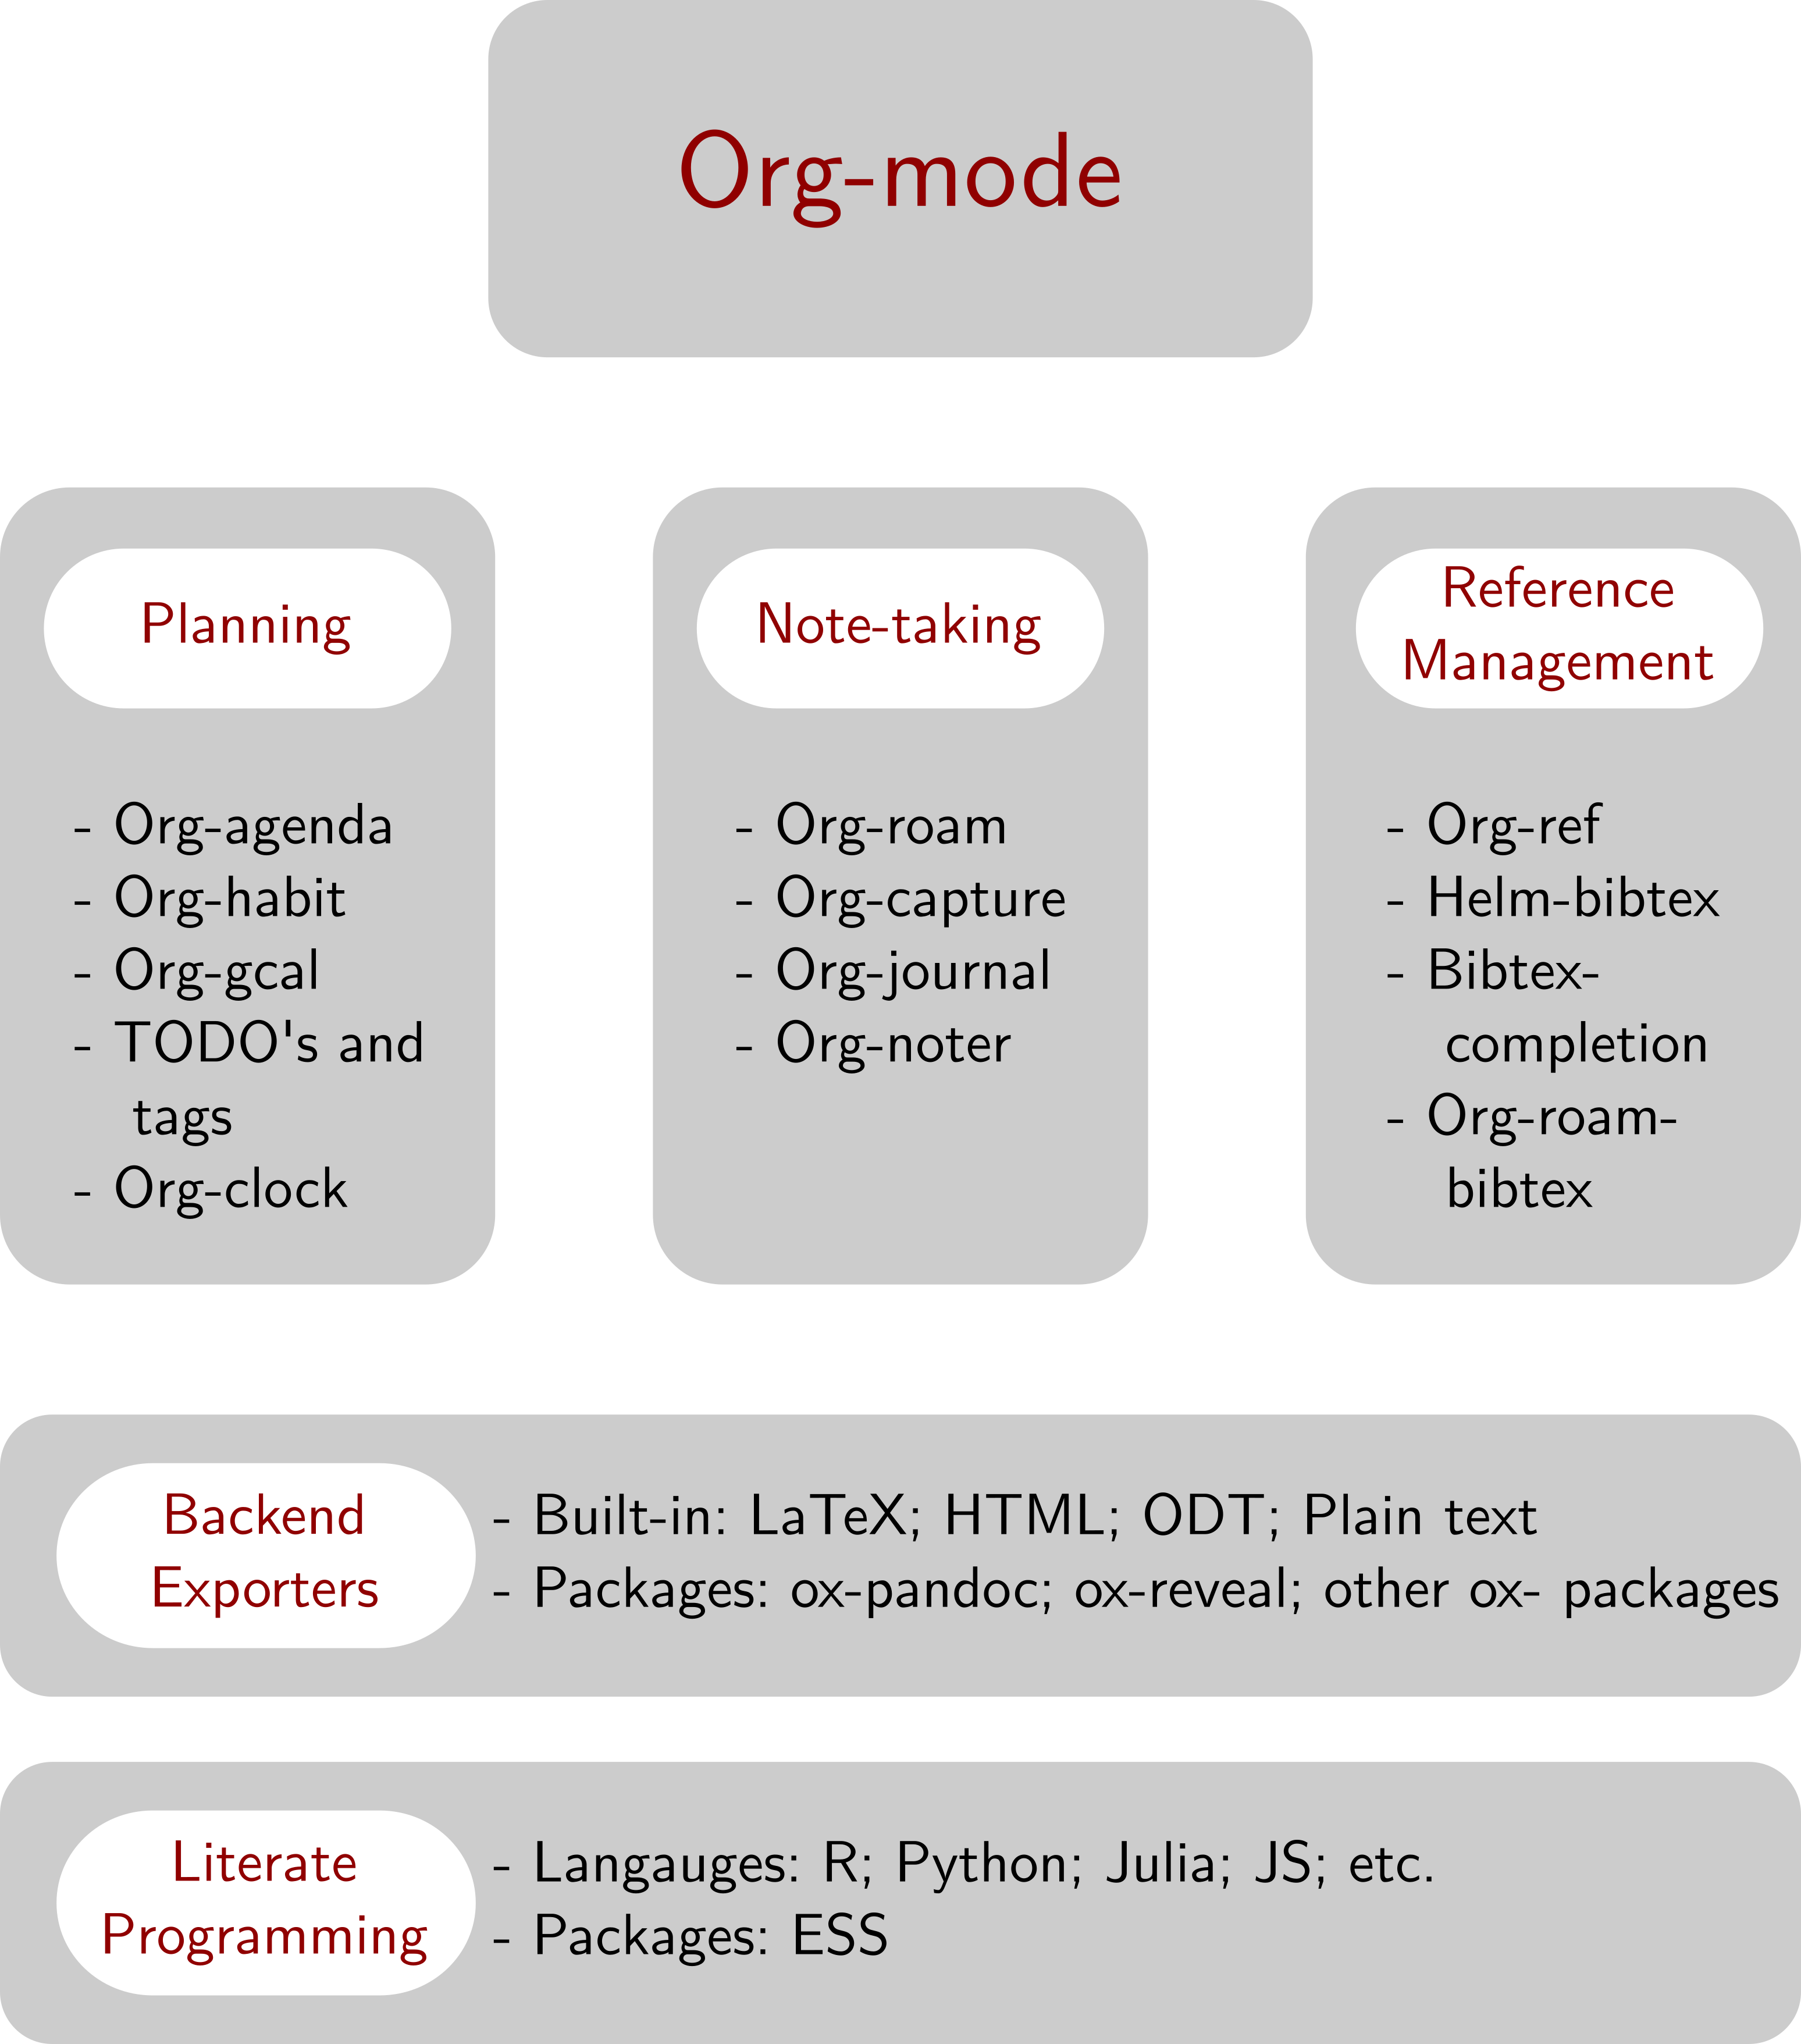
\includegraphics[width=0.5\textwidth]{org-mode.png}
\end{center}
\end{frame}



\begin{frame}[label={sec:org74ff8ab},fragile]{Org-mode}
 I use org files to conduct most of my literate programming and create documents that are exportable into other formats such as \texttt{.tex}, \texttt{.docx}, \texttt{.html}, and many more. For example, this presentation was created in an org file, and I used LaTeX's beamer class to export it into PDF.

\begin{center}
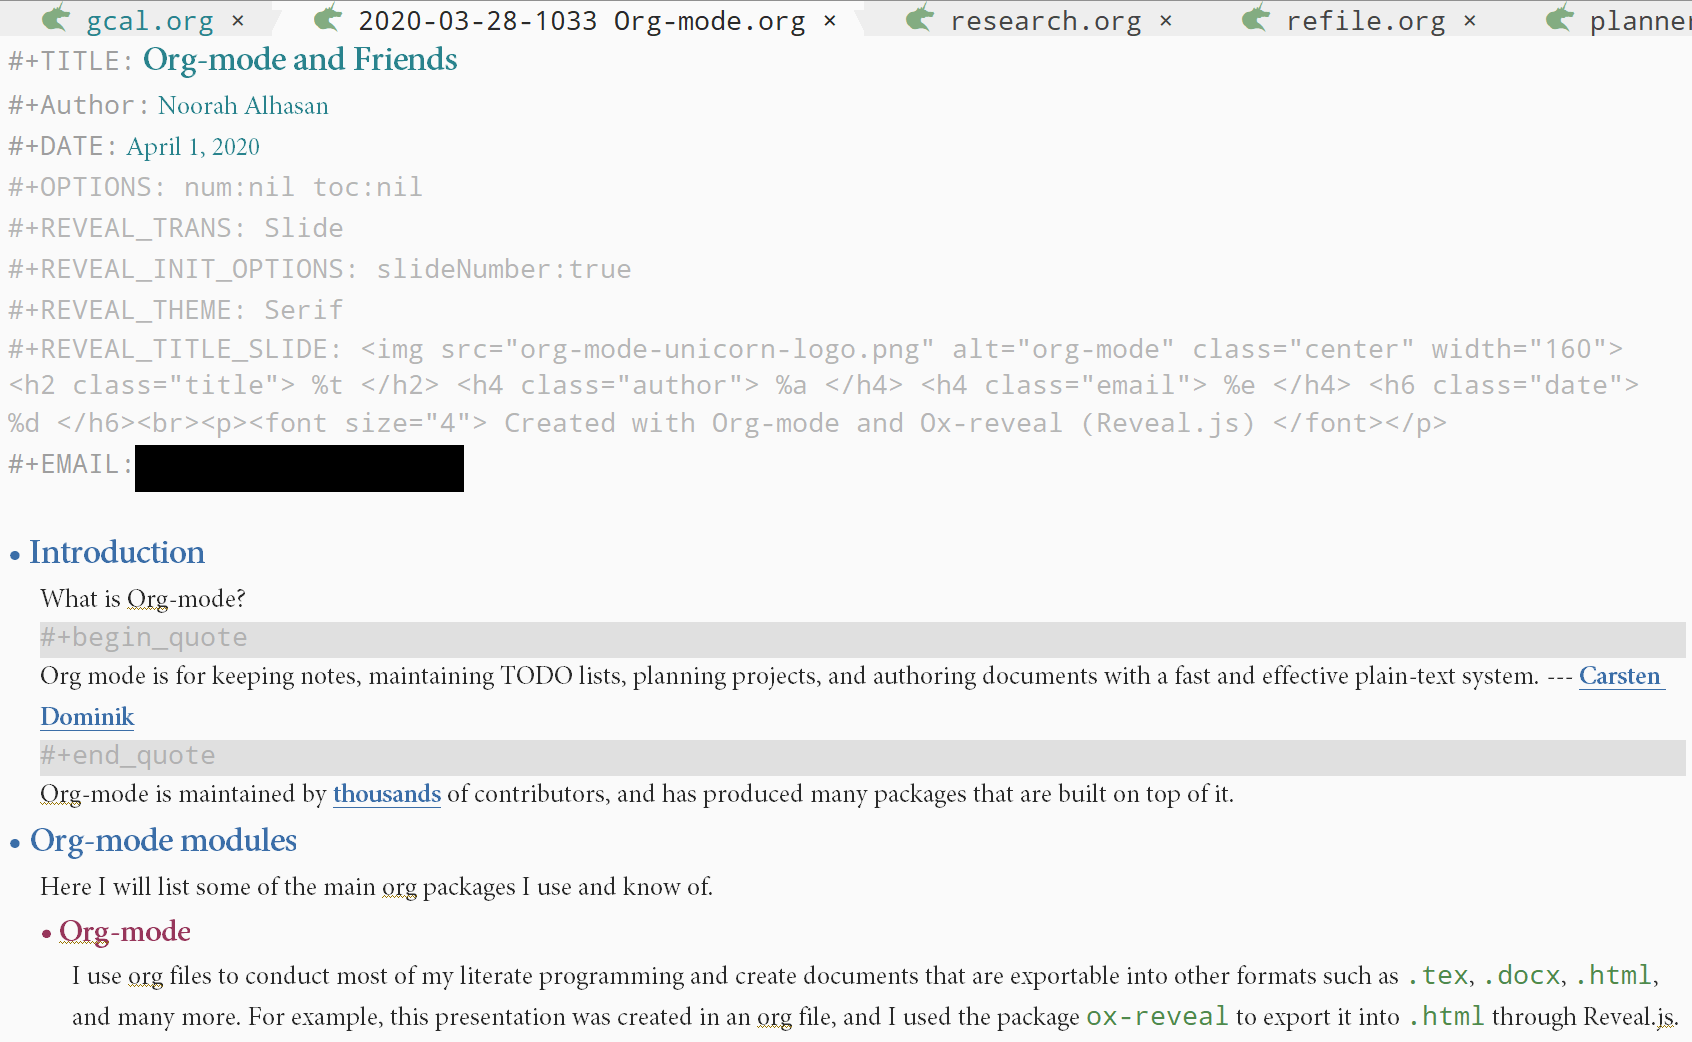
\includegraphics[width=0.65\textwidth]{c:/Users/Noorah/Dropbox/emacs projects/2020-03-28-1033 Org-mode.org_20200329_164548_clXDXk.png}
\end{center}
\end{frame}

\begin{frame}[label={sec:orgb0aab8f},fragile]{Org-agenda}
 \small
\begin{itemize}
\item Populates all your \texttt{TODO} s and appointments into a singular view.
\item You can add an org-file into the agenda using ``\texttt{C-c [}'' in the current org-file.
\item There are many views in the org-agenda, and the default is week-view.
\item You can also customize an org-agenda using \texttt{org-agenda-custom-commands}, or use packages such \texttt{org-super-agenda}.
\item I set up my agenda as a daily view with appointments, deadlines, and a habit tracker.
\end{itemize}

\begin{center}
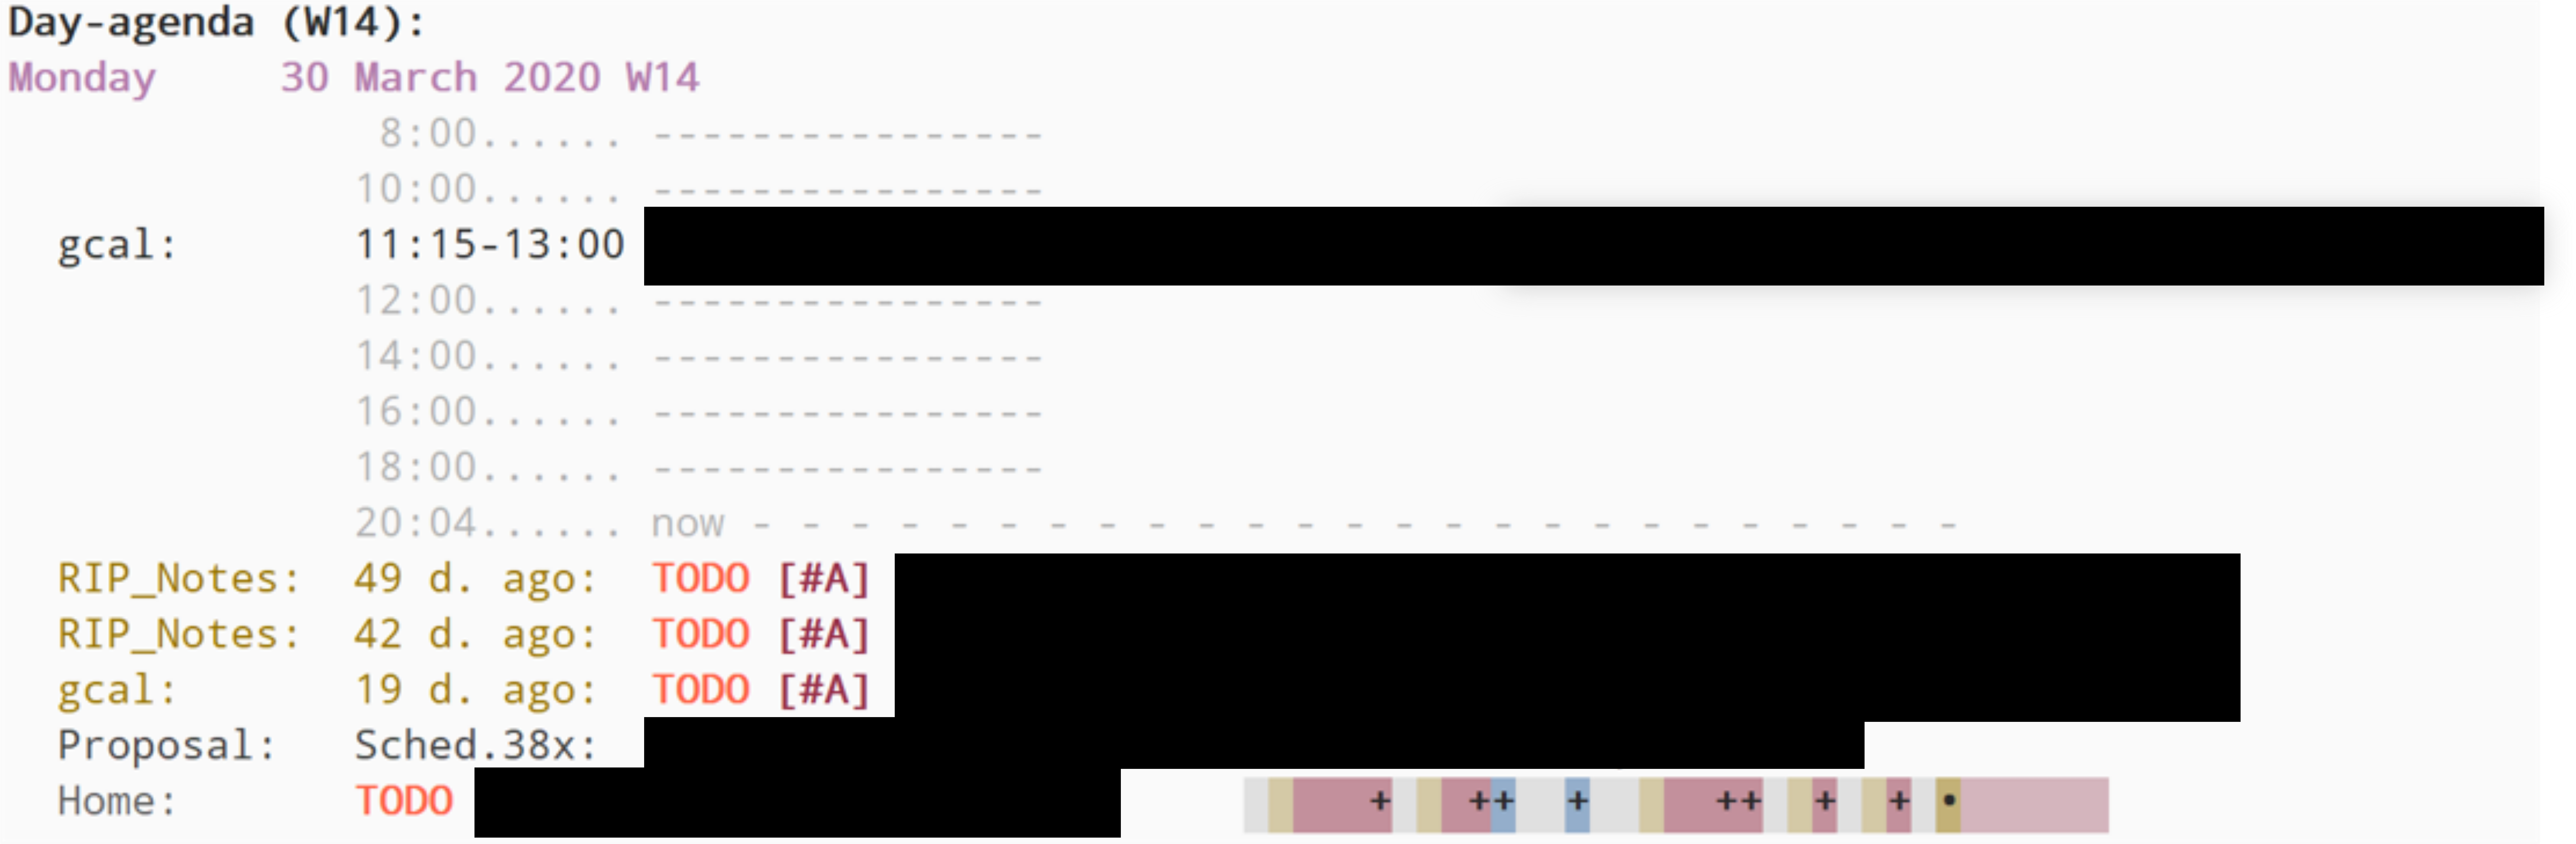
\includegraphics[width=0.65\textwidth]{5.png}
\end{center}
\end{frame}

\begin{frame}[label={sec:org3c05022}]{Org-gcal}
Package that syncs all your Google calendar entries with org-mode, which you can then add the org-file to the agenda.
\end{frame}

\begin{frame}[label={sec:orgb456ecb}]{Org-habit}
A package to produce a nice visual for recurring tasks, i.e. habits, that you can also have appearing in your agenda.

\begin{center}
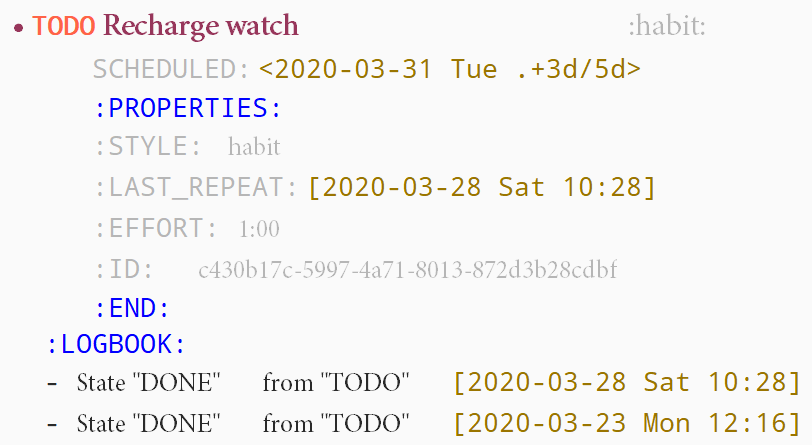
\includegraphics[width=0.75\textwidth]{c:/Users/Noorah/Dropbox/orgfiles/planner.org_20200401_105921_boLAcS.png}
\end{center}
\end{frame}

\begin{frame}[label={sec:org93dc8a8},fragile]{\texttt{TODO} 's and tags}
 \begin{itemize}
\item These are identifiers in an org-file as tasks or reminders.
\item The types of \texttt{TODO} s can either be set globally in your init file, or they can be file specific.
\item They can also be placed as a subtree, or in-line (\texttt{'org-inlinetask}).
\item You can assign deadlines, scheduled date and time, active timestamps, and inactive timestamps.
\end{itemize}

\begin{itemize}
\item \alert{Deadlines}: \texttt{TODO} must be completed at a certain date and time. Date is mandatory but time is optional.
\item \alert{Scheduled}: Must start task on a certain date and time.
\item \alert{Active timestamp}: Behaves like an appointment.
\item \alert{Inactive timestamp}: shows under the task but does not appear in the agenda.
\end{itemize}
\end{frame}

\begin{frame}[label={sec:orgf37dc3c},fragile]{\texttt{TODO} 's and tags}
 \begin{center}
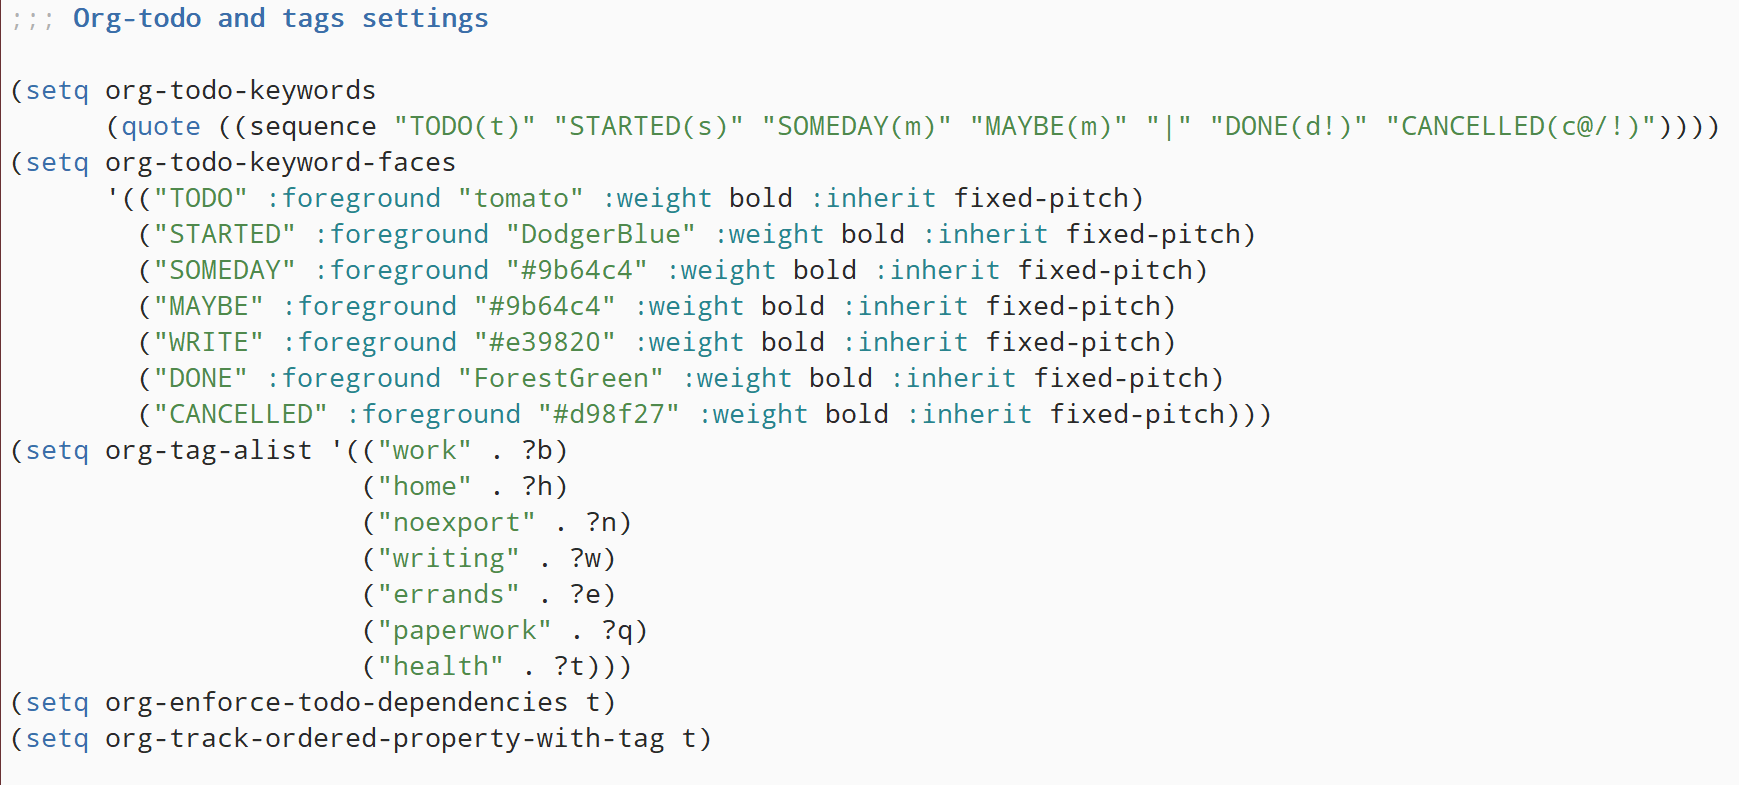
\includegraphics[width=0.85\textwidth]{c:/Users/Noorah/Dropbox/emacs projects/init.el_20200329_180056_xitTr0.png}
\end{center}
\end{frame}

\begin{frame}[label={sec:org205d431},fragile]{\texttt{TODO} 's and tags}
 \begin{center}

\includegraphics[width=0.85\textwidth]{c:/Users/Noorah/Dropbox/emacs projects/Proposal.org_20200329_182231_vvs3sT.png}
\end{center}
\end{frame}

\begin{frame}[label={sec:orge338c7e},fragile]{Properties drawer}
 \begin{itemize}
\item Each org heading, also called a subtree, within an org file can have certain properties.
\begin{itemize}
\item For example, you can assign a unique \texttt{ID} (\texttt{org-id-get-create}) that is searchable, refiled, or hyperlinked throughout emacs, create a specific org-export filename for that subtree, or add any other configuration that is subtree specific.
\end{itemize}
\end{itemize}
\end{frame}

\begin{frame}[label={sec:org3820805}]{Properties drawer}
\begin{center}
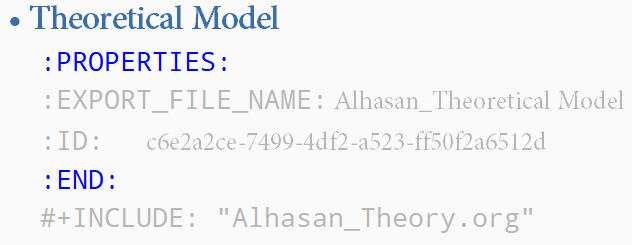
\includegraphics[width=0.75\textwidth]{c:/Users/Noorah/Dropbox/emacs projects/Proposal.org_20200330_192520_cqrX8N.png}
\end{center}
\end{frame}

\begin{frame}[label={sec:org90d6136}]{Properties drawer}
\begin{center}
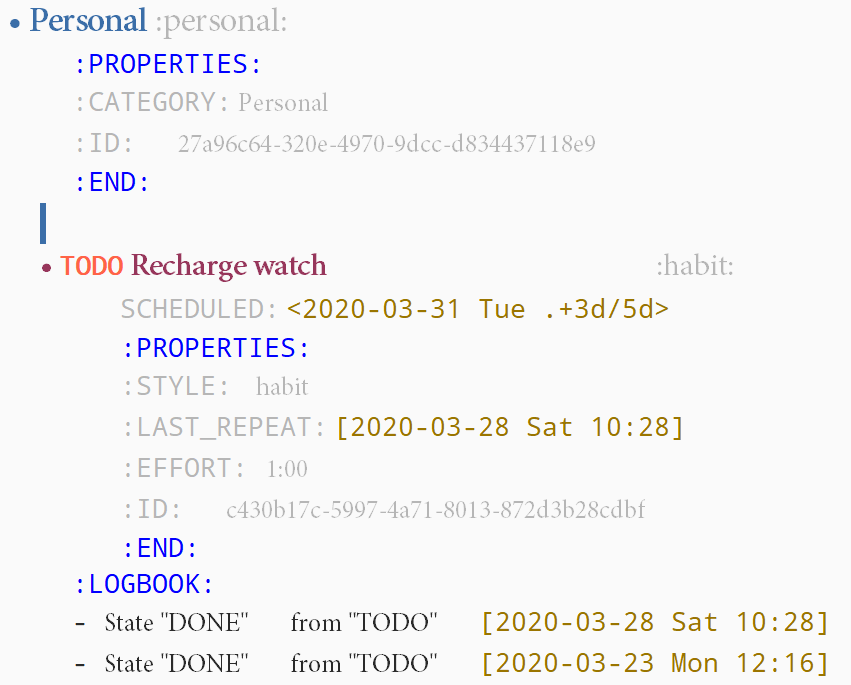
\includegraphics[width=0.75\textwidth]{3.png}
\end{center}
\end{frame}

\begin{frame}[label={sec:org045d056},fragile]{Org-clock}
 Last time we briefly talked about org-clock, which is basically clocking any of your current tasks. To invoke clocking a task requires two things:

\begin{enumerate}
\item An org-heading.
\item An \texttt{:EFFORT:} property set for a length of time.
\end{enumerate}

I've customized my org-clock setting such that the minute I clock into a task, it switches the state of the heading to \texttt{STARTED}, so it can appear in my agenda.
\end{frame}

\begin{frame}[label={sec:org3fb2a23},fragile]{Org-roam}
 A note-taking package that replicates Roam Research which is based on the Zettelkasten method. I use it to build my literature review and I use \texttt{org-roam-server} to visualize my notes into a network.


\begin{center}
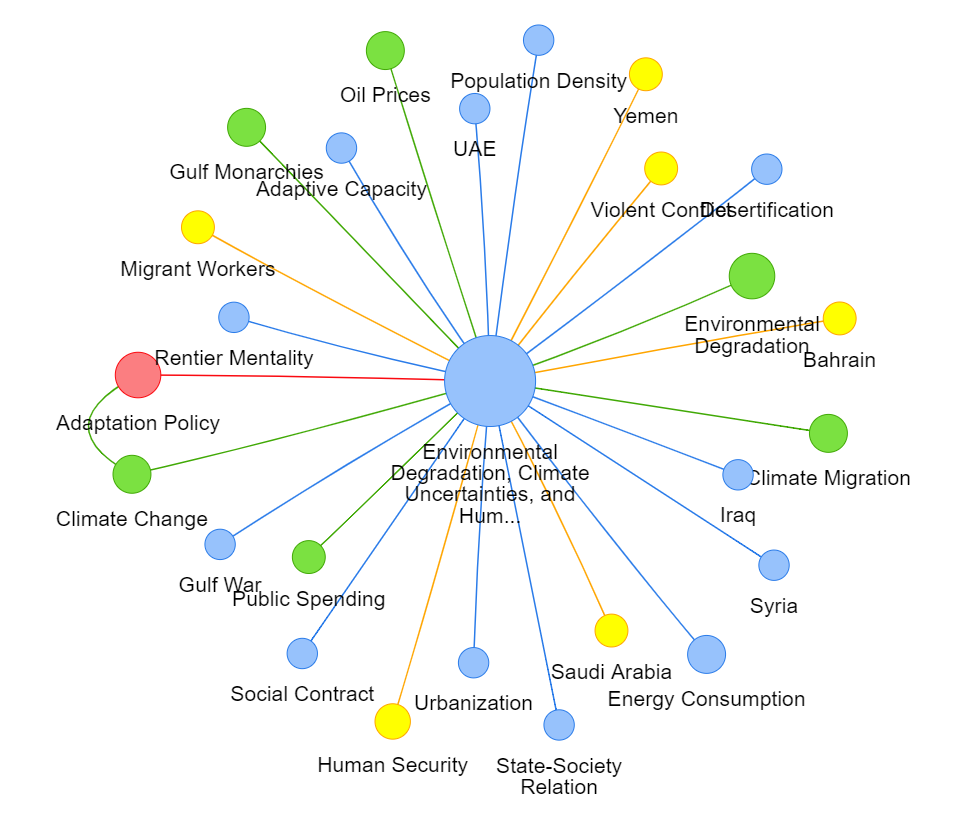
\includegraphics[width=0.65\textwidth]{7.png}
\end{center}
\end{frame}

\begin{frame}[label={sec:org317d231},fragile]{Org-capture}
 These are customizable org-headings that you can create on-the-go. They can be regular \texttt{TODO} s or just notes.

\begin{center}
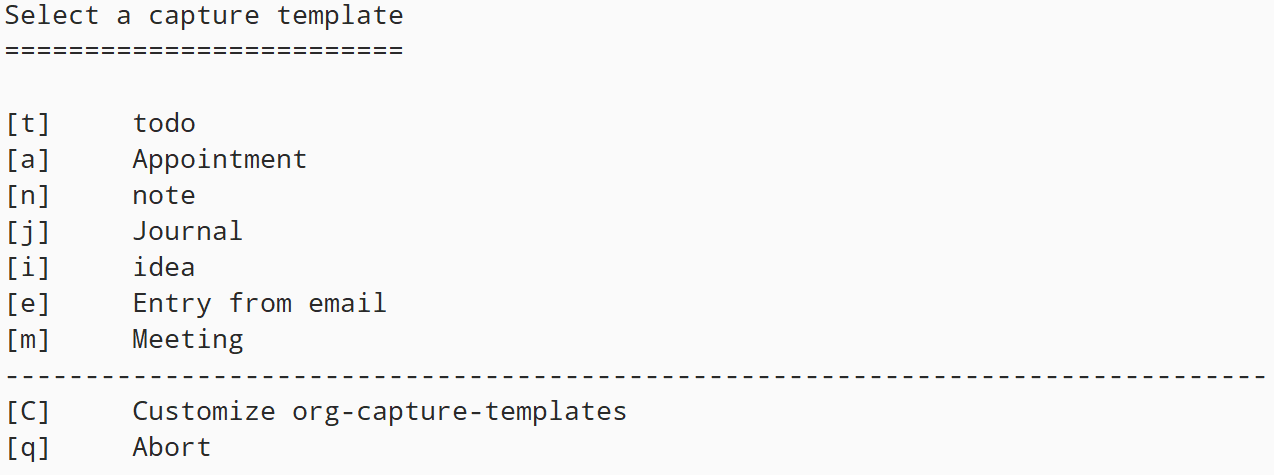
\includegraphics[width=0.75\textwidth]{6.png}
\end{center}
\end{frame}

\begin{frame}[label={sec:orgf5b8704},fragile]{Org-noter}
 \begin{itemize}
\item I use it to annotate PDFs and take notes within the same buffer.
\begin{itemize}
\item It uses the \texttt{interleave} package to locate the PDF document and \texttt{PDF-tools} for the annotation tools such as highlighting.
\end{itemize}
\end{itemize}

\begin{center}
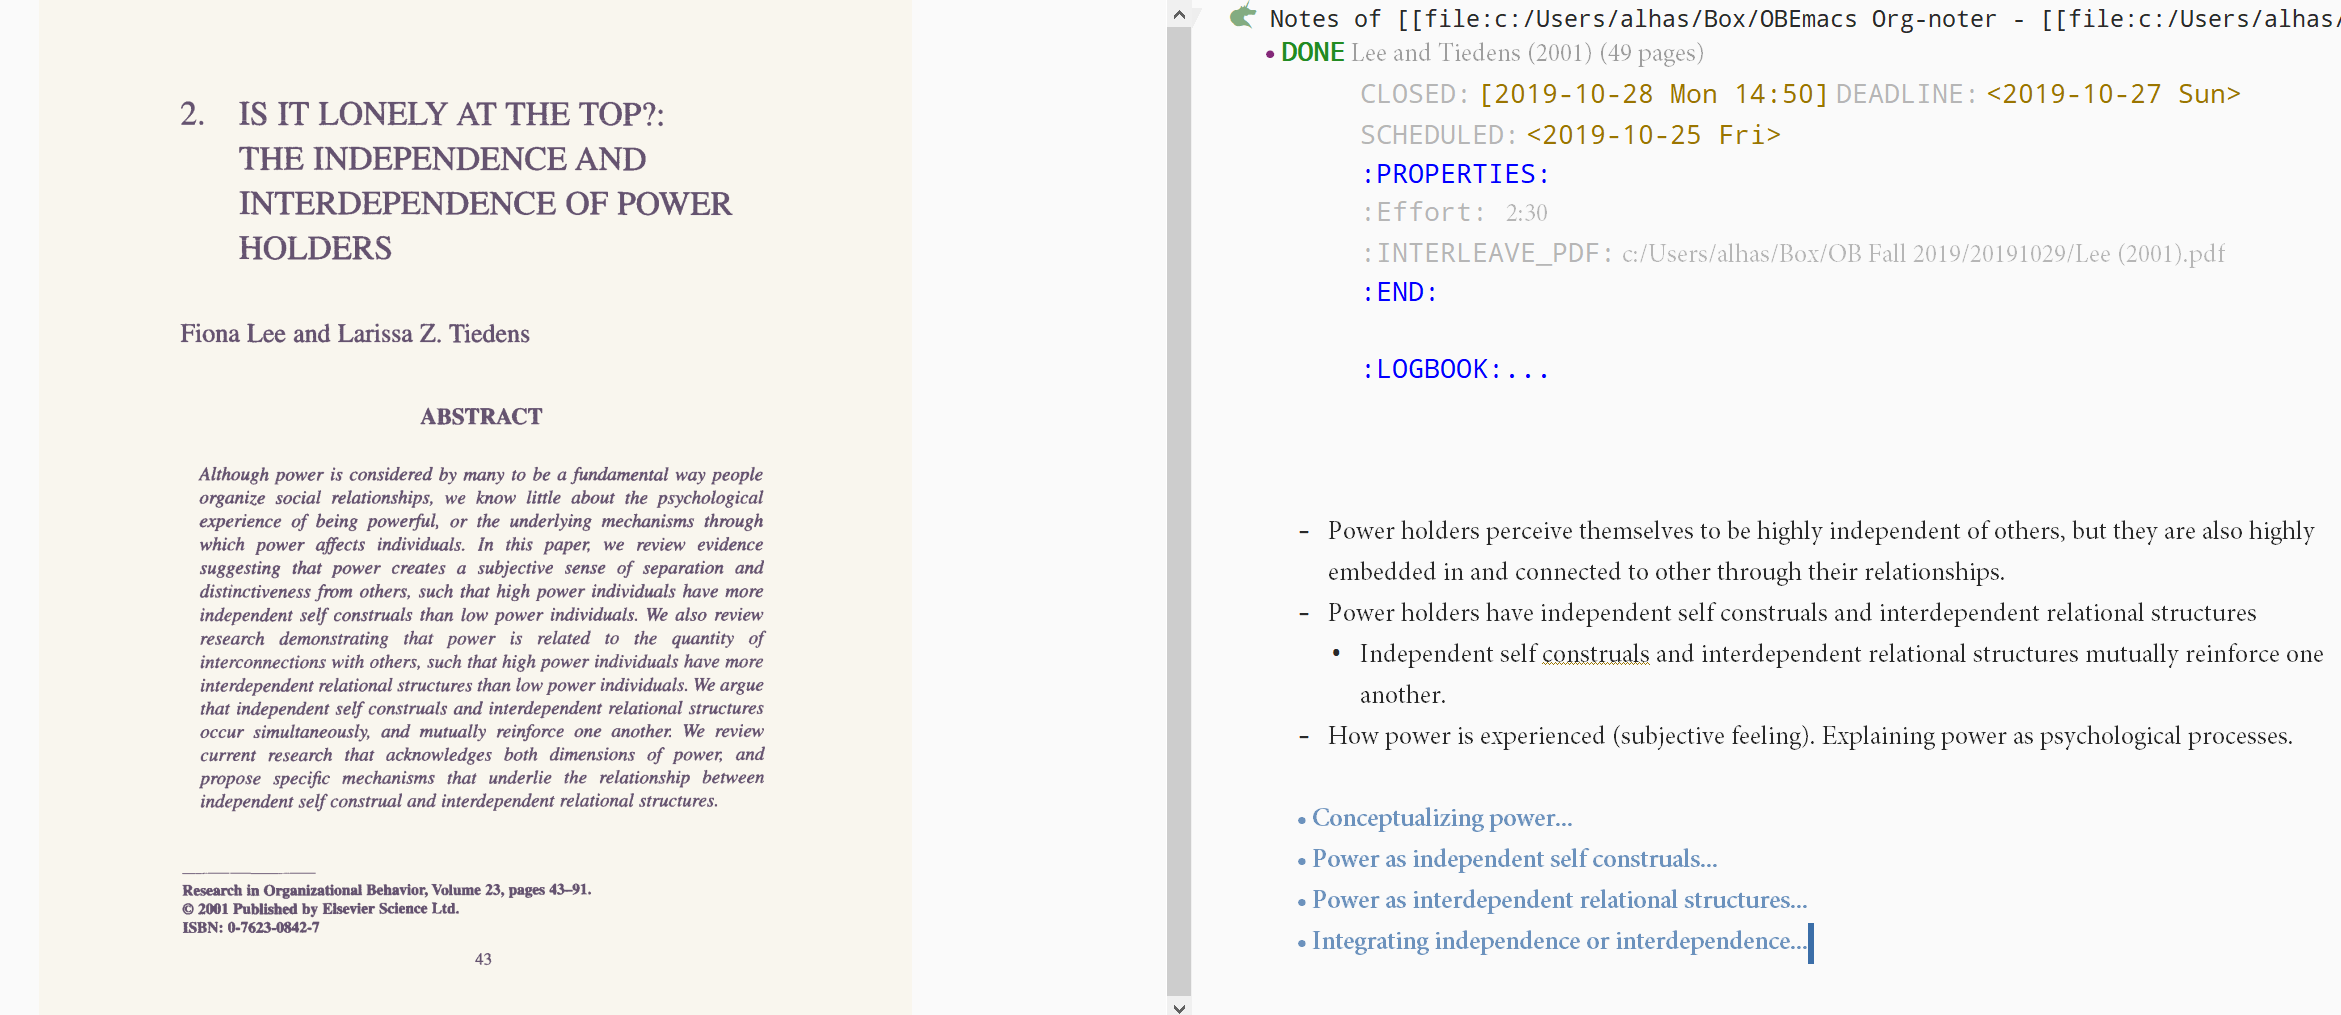
\includegraphics[width=\textwidth]{c:/Users/Noorah/Dropbox/orgfiles/Archive/Fall 2019/OB_Notes.org_20200401_124730_u6JqKp.png}
\end{center}
\end{frame}

\begin{frame}[label={sec:org1edb5de},fragile]{Org-ref}
 \begin{itemize}
\item I started out with \texttt{org-ref}, and I still use some of its command especially with citation styles.
\item You can add references to your master \texttt{.bib} file straight into emacs and can cite references in any org file within emacs.
\item I have all my references in one bib file so I don't have to specify a bib file in each org-buffer, but it also allows other bib files as long as you invoke them within an org file.
\end{itemize}
\end{frame}

\begin{frame}[label={sec:org143078c},fragile]{Org-roam-bibtex}
 Utilizes a combination of \texttt{org-ref}, \texttt{helm-bibtex}, and \texttt{bibtex-completion} to streamline note-taking workflow with references within the \texttt{org-roam} ecosystem.
\end{frame}
\begin{frame}[label={sec:org715788e},fragile]{Exporters}
 Default org-mode exporter include \texttt{.tex}, \texttt{.pdf}, \texttt{.odt}, and \texttt{.html}. Other backend org-exporters include packages such as \texttt{ox-pandoc}, \texttt{ox-reveal}, and \texttt{ox-hugo}.

There are many other ox- packages but the previous three are the ones I use, especially ox-pandoc, because it exports to many other formats, such as \texttt{.docx} (useful to share documents with people that only work with WYSIWG text editors).
\end{frame}

\begin{frame}[label={sec:org658897e}]{Exporters}
\begin{center}
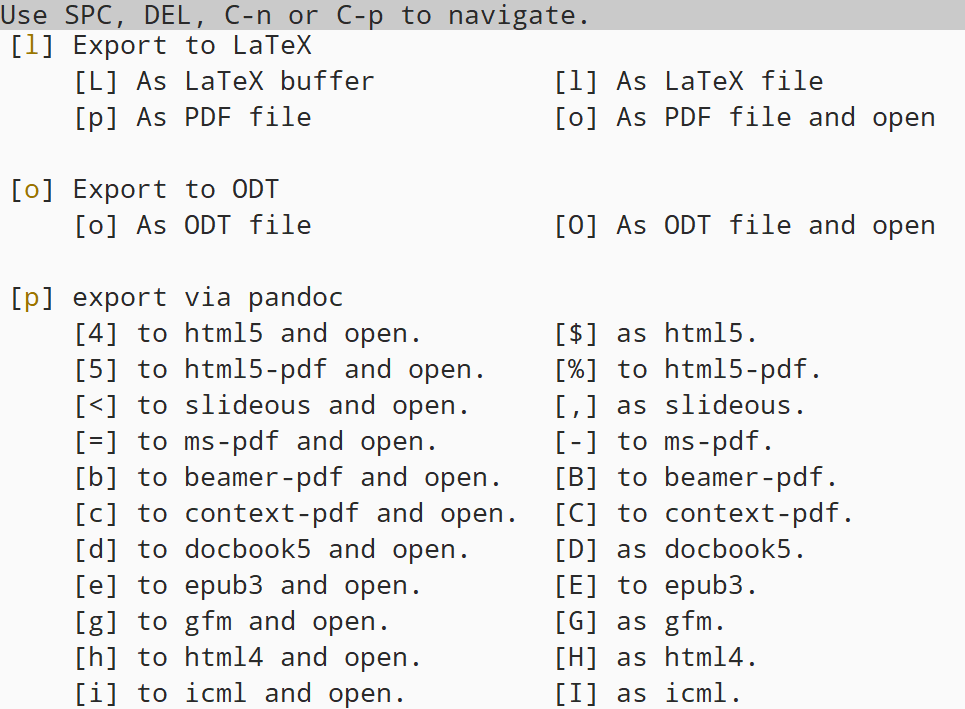
\includegraphics[width=0.65\textwidth]{4.png}
\end{center}
\end{frame}

\begin{frame}[label={sec:org134bdd5}]{Org-babel}
This package is for code execution within org-mode files. Basically, literate programming.
\end{frame}

\begin{frame}[label={sec:org6dd305d}]{Org-babel}
\begin{center}
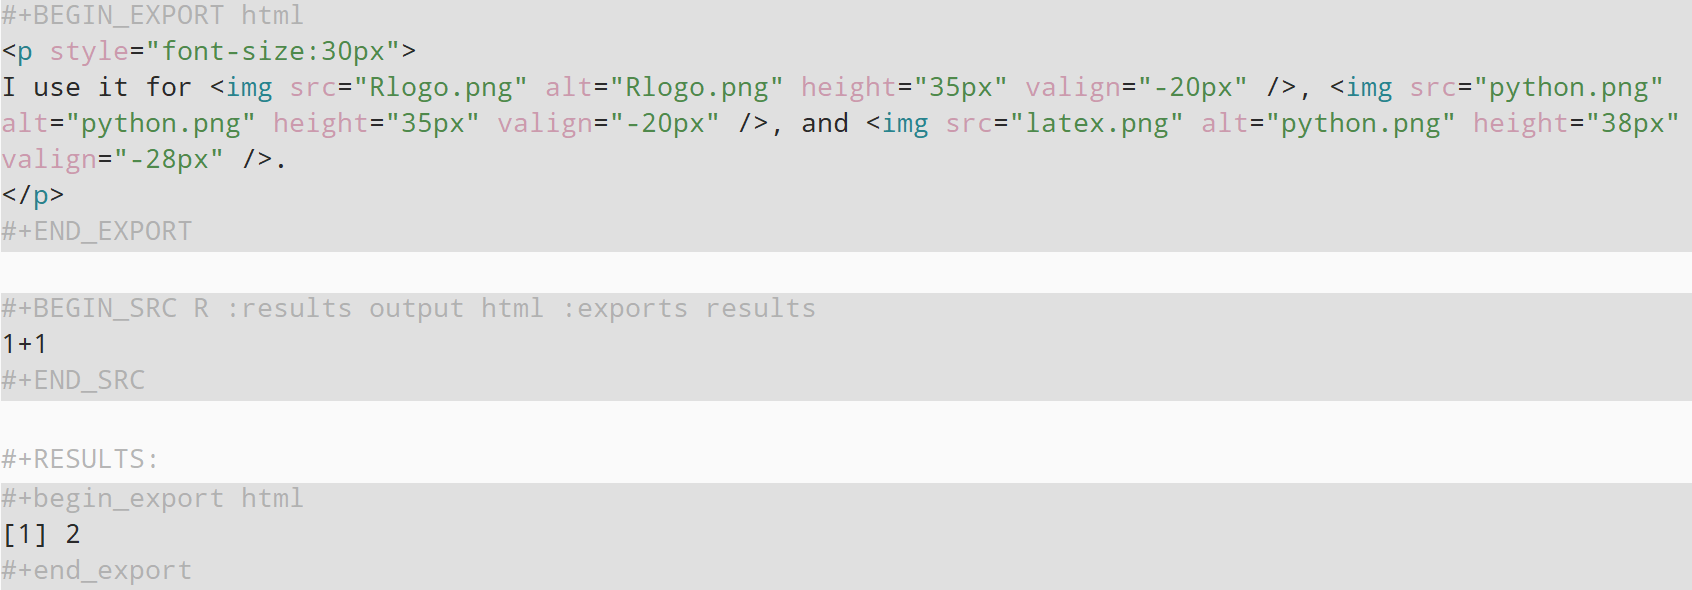
\includegraphics[width=0.85\textwidth]{c:/Users/Noorah/Dropbox/emacs projects/2020-03-28-1033 Org-mode.org_20200330_210612_Sa67q6.png}
\end{center}
\end{frame}
\end{document}
